We consider the one-dimensional heat equation with Dirichlet, Neumann, and periodic boundary conditions, discretized on a two-qubit register. Unless otherwise stated, the numerical target is the exact discretized solution vector $u(T)=e^{-AT}u(0)$ at total evolution time $T=1$, with oscillator truncation $n_{\mathrm{fock}}=64$ and first-order Trotterization using $n_{\mathrm{trotter}}=100$ steps.

For the numerical study we fix a four-dimensional semidiscrete system encoded on a two-qubit register, with $M=4$, $\alpha=1$, $h=1$, $T=1$, and initial state $u(0)=\ket{01}$. Since $\alpha/h^2=1$ in all three cases, the exact semidiscrete generators used in the simulations are
{\small
\[
\begin{aligned}
A^{(\mathrm D)}&=
\begin{bmatrix}
2&-1&0&0\\
-1&2&-1&0\\
0&-1&2&-1\\
0&0&-1&2
\end{bmatrix},
&&u(0,t)=u(\mathcal L,t)=0,\\[0.5em]
A^{(\mathrm N)}&=
\begin{bmatrix}
1&-1&0&0\\
-1&2&-1&0\\
0&-1&2&-1\\
0&0&-1&1
\end{bmatrix},
&&\partial_x u(0,t)=\partial_x u(\mathcal L,t)=0,\\[0.5em]
A^{(\mathrm P)}&=
\begin{bmatrix}
2&-1&0&-1\\
-1&2&-1&0\\
0&-1&2&-1\\
-1&0&-1&2
\end{bmatrix},
&&u(0,t)=u(\mathcal L,t),\ \partial_x u(0,t)=\partial_x u(\mathcal L,t).
\end{aligned}
\]
}

For normalized states, fidelities are reported as
\[
F(\psi,\phi)=|\langle \psi \mid \phi\rangle|^2
\]
and the exact semidiscrete target is
\[
u_{\mathrm{exact}}(T)=e^{-AT}u(0).
\]
We use
\[
F_{\mathrm{exact}}=F(u_{\mathrm{alg}},u_{\mathrm{exact}}),\qquad
F_{\mathrm{trunc}}=F(u_{\mathrm{alg}},u_{\mathrm{trunc}}),\qquad
F_{\mathrm{oracle}}=F(\psi_{\mathrm{prep}},\psi_{\mathrm{target}}),
\]
where $u_{\mathrm{trunc}}$ is the exact finite-Fock reference induced by the same kernel parameters and $\psi_{\mathrm{target}}$ is the ideal truncated oscillator state. The quantities $F_{\mathrm{snap}}$, $F_{\mathrm{givens}}$, and $F_{\mathrm{DV}}$ denote the end-to-end PDE fidelities obtained with SNAP$+$D, Givens preparation, and the classical DV LCHS quadrature, respectively. The CV postselection probability is
\[
p_{\mathrm{post}}
 :=
\left\|
(\langle 0|\,S^\dagger(r_{\mathrm{target}})\otimes I)\,\Psi_{\mathrm{out}}
\right\|^2 .
\]
The quantity $n_{\mathrm{coeff}}$ denotes the number of retained oscillator Fock amplitudes in the truncated CV oracle state,
\[
\psi_{\mathrm{target}} \approx \sum_{n=0}^{n_{\mathrm{coeff}}-1} c_n \ket{n}.
\]

\subsection{Parameter selection}

Injection-based parameter sweeps are used to select the kernel parameters $r_{\mathrm{target}}$, $r^\prime$, and $\beta$. Since the CV resource state is loaded ideally, these data isolate kernel quality rather than gate-level state-preparation error. The overall search domain covered
\[
r_{\mathrm{target}}\in[1.92,8.4],\qquad
r^\prime\in[0.975,4.5],\qquad
\beta\in[0.3,0.9],
\]
with $n_{\mathrm{coeff}}\in\{24,48\}$ and $n_{\mathrm{trotter}}=100$. The highest-fidelity region was then sampled more densely on the intervals $r_{\mathrm{target}}\in[7.8,8.4]$ and $r^\prime\in[4.0,4.5]$, which is the domain represented in Fig.~\ref{fig:clean_sensitivity_exact}. For each displayed value of a given parameter, the plotted point is the best exact fidelity obtained while that parameter is held fixed and the remaining parameters vary over the tested grid.

Across all three boundary conditions, the oracle-baseline optima lie in a narrow high-squeezing region. Dirichlet is optimized at $(r_{\mathrm{target}},r^\prime,\beta,n_{\mathrm{coeff}})=(7.9,4.1,0.5,48)$, Neumann at $(7.9,4.0,0.3,48)$, and periodic at $(8.1,4.1,0.3,48)$, with exact fidelities above $0.9989$ in all three cases.

\begin{figure}[h]
\centering
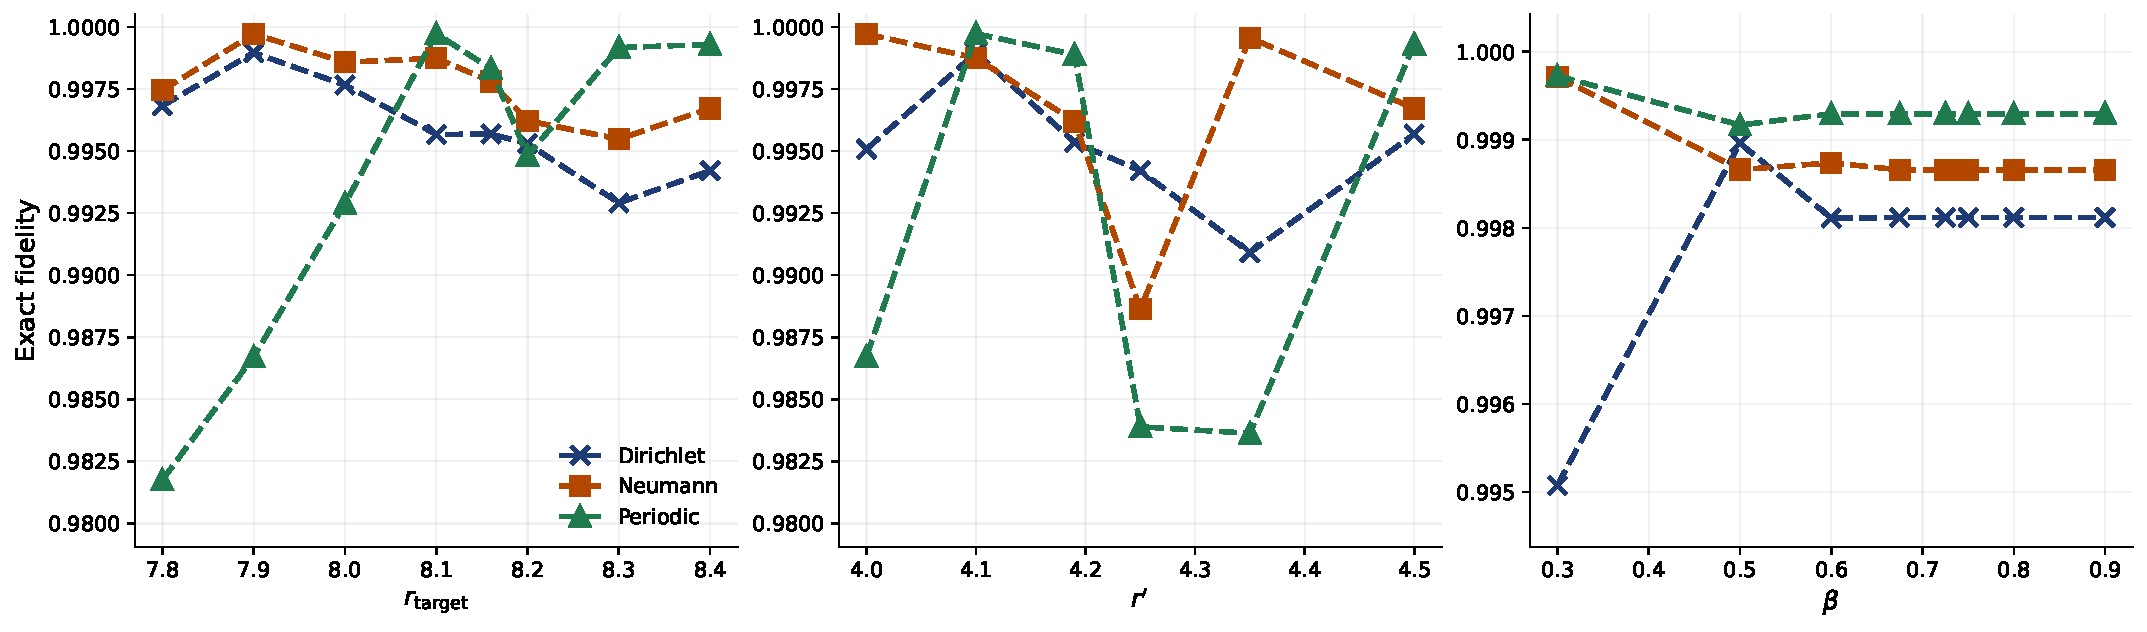
\includegraphics[width=\linewidth]{Pics/section6_sensitivity_exact.pdf}
\caption{Sensitivity of the exact PDE fidelity to the kernel parameters under ideal CV loading, shown for the denser high-fidelity subdomain $r_{\mathrm{target}}\in[7.8,8.4]$ and $r^\prime\in[4.0,4.5]$. The three panels show, from left to right, variation with $r_{\mathrm{target}}$, $r^\prime$, and $\beta$. For each plotted value on the horizontal axis, the vertical coordinate is the best exact fidelity obtained while the remaining sweep parameters vary over the tested grid.}
\label{fig:clean_sensitivity_exact}
\end{figure}

\begin{table}[h]
\centering
\caption{Parameter choices from the ideal-loading sweep, together with the corresponding fidelities $F_{\mathrm{exact}}$ and $F_{\mathrm{trunc}}$. Here $F_{\mathrm{exact}}$ is measured against the discretized heat-equation solution vector and $F_{\mathrm{trunc}}$ against the finite-Fock CV reference.}
\label{tab:clean_oracle_baseline}
\begin{tabular}{lccccccc}
\toprule
Boundary & $r_{\mathrm{target}}$ & $r^\prime$ & $\beta$ & $n_{\mathrm{coeff}}$ & $F_{\mathrm{exact}}$ & $F_{\mathrm{trunc}}$ & $p_{\mathrm{post}}$ \\
\midrule
Dirichlet & 7.9 & 4.1 & 0.5 & 48 & 0.998961 & 0.999992 & 0.06279 \\
Neumann & 7.9 & 4.0 & 0.3 & 48 & 0.999716 & 0.999984 & 0.05616 \\
Periodic & 8.1 & 4.1 & 0.3 & 48 & 0.999725 & 1.000000 & 0.04842 \\
\bottomrule
\end{tabular}
\end{table}

\subsection{Empirical relation to the theoretical bounds}

Theorem~\ref{thm: state-prep} is asymptotic and contains unspecified constants $\mathcal K$ and $\mathcal M$, which collect the prefactors in the truncation and squeezing estimates. The experiments therefore test qualitative consistency rather than calibrated numerical tightness. Across the ideal-loading parameter study, increasing the oscillator coefficient cutoff from $n_{\mathrm{coeff}}=24$ to $48$ improves the best exact fidelity in all three cases: Dirichlet from $0.9956816$ to $0.9989611$, Neumann from $0.9995599$ to $0.9997155$, and periodic from $0.9992957$ to $0.9997249$. This trend is consistent with Theorem~\ref{thm: state-prep}, which predicts improved approximation as the truncated oscillator resources increase. The same data place the optimum in a large-squeezing regime, with both $r_{\mathrm{target}}$ and $r^\prime$ near $4$ to $8$, again in qualitative agreement with the squeezing dependence of the theorem.

For the hybrid evolution, Eq.~\eqref{eq:heat-trotter-error} predicts first-order scaling in the number of product-formula steps. Using the Dirichlet data and comparing against the truncated CV reference rather than the exact PDE solution, the best observed relative errors are $3.0835\times 10^{-3}$ at $n_{\mathrm{trotter}}=8$, $1.5428\times 10^{-3}$ at $n_{\mathrm{trotter}}=16$, and $7.7171\times 10^{-4}$ at $n_{\mathrm{trotter}}=32$. These values follow a normalized $C/n$ guide line closely, providing a representative empirical check of the expected first-order behavior. This quantitative tightness check is available only for the low-to-moderate Dirichlet sweep region, rather than for the highest-fidelity operating points or uniformly across all three boundary conditions.


\subsection{End-to-end fidelity and state-preparation effects}

Table~\ref{tab:clean_snap_comparison} compares Givens synthesis and SNAP$+$D preparation at the parameter values listed in Table~\ref{tab:clean_oracle_baseline}. In all three cases, the SNAP$+$D row uses the best depth identified by the state-preparation study at the corresponding kernel point.

The data show that the optimized SNAP$+$D circuits now close the gap to the ideal baseline in all three boundary conditions. The Neumann and periodic cases are closest to the Givens reference, with differences of $3.78\times 10^{-5}$ and $1.94\times 10^{-4}$, respectively. Dirichlet also remains close, with $F_{\mathrm{snap}}=0.996817$ and a difference of $2.14\times 10^{-3}$.

\begin{table}[h]
\centering
\caption{Givens and SNAP$+$D fidelity comparison at the parameter values in Table~\ref{tab:clean_oracle_baseline}. In all three cases, the SNAP$+$D row uses the best depth identified at the corresponding kernel point.}
\label{tab:clean_snap_comparison}
\begin{tabular}{lcccr}
\toprule
Boundary & $F_{\mathrm{givens}}$ & $F_{\mathrm{snap}}$ & $F_{\mathrm{oracle}}$ & Depth \\
\midrule
Dirichlet & 0.998961 & 0.996817 & 0.994380 & 30 \\
Neumann & 0.999716 & 0.999678 & 0.995048 & 30 \\
Periodic & 0.999725 & 0.999531 & 0.996856 & 30 \\
\bottomrule
\end{tabular}
\end{table}

\subsection{Physical interpretation and resource costs}

The high-fidelity oracle-baseline points occur at large values of $r_{\mathrm{target}}$ and $r^\prime$. In the CV-DV LCHS construction, the ancillary oscillator enters through the qumode sandwich $\langle \phi | e^{-it(\hat{x}\otimes L + I\otimes H)} | \psi \rangle$, so these high-squeezing values indicate that the CV resource state must realize a sufficiently broad quadrature-space kernel profile over the relevant spectral window of $A$. The corresponding gain in exact PDE fidelity is accompanied by a smaller postselection probability. At the same time, $F_{\mathrm{trunc}}$ remains essentially unity, showing that once the oscillator seed state is fixed, the hybrid evolution tracks the finite-Fock target very accurately.

The distinction among $F_{\mathrm{oracle}}$, $F_{\mathrm{snap}}$, and $F_{\mathrm{trunc}}$ is physically informative. The quantity $F_{\mathrm{oracle}}$ measures only how accurately SNAP$+$D reproduces the target oscillator seed. The quantity $F_{\mathrm{snap}}$ measures the final PDE solution fidelity, and $F_{\mathrm{trunc}}$ measures agreement with the exact finite-Fock evolution generated by the prepared seed itself. Consequently, $F_{\mathrm{trunc}}\approx 1$ together with a smaller $F_{\mathrm{oracle}}$ shows that the hybrid evolution is accurate once the prepared state is fixed, so the remaining discrepancy is attributable to state preparation rather than to the subsequent CV-DV dynamics. The present data indicate that this state-preparation gap can be made small in all three cases. For Dirichlet, Neumann, and periodic boundary conditions, the optimized SNAP$+$D circuits reach $F_{\mathrm{oracle}}=0.994380$, $0.995048$, and $0.996856$, with corresponding end-to-end fidelities $F_{\mathrm{snap}}=0.996817$, $0.999678$, and $0.999531$. Thus the practical implementation is now close to the ideal oracle baseline across all three benchmarks.

Givens synthesis furnishes an analytic exact-synthesis baseline together with JC-pulse and qubit-rotation counts. In all three boundary conditions, Givens matches the injection fidelity to numerical precision while reporting 47 JC pulses and 47 qubit rotations.

For the hybrid evolution block itself, the gate structure is simpler than the total circuit depth might suggest. From the standpoint of implementation difficulty, the relevant CV operations are Gaussian single-mode gates, hybrid controlled Gaussian gates, and non-Gaussian state-preparation gates. In the present circuits, the 100-step Trotterized CV-DV evolution uses only qubit single-qubit basis-change gates, CNOT ladders, unconditional displacements $D(\alpha)$, and qubit-controlled displacements, denoted below by $CD$. The two squeezing gates that form the outer kernel sandwich are fixed Gaussian one-mode overheads, while the SNAP$+$D routine contributes the non-Gaussian part of the oracle preparation. Here one $\mathrm{SNAP}_{48}+D$ layer means a SNAP gate with 48 active number-state phases, followed by one displacement gate. By contrast, direct state loading is used only for the ideal oracle baseline and is not counted as a gate-synthesis primitive.

\begin{table}[h]
\centering
{\small
\caption{Representative resource counts for the SNAP$+$D circuits in Table~\ref{tab:clean_snap_comparison} and for the analytic Givens baseline. The Trotter columns refer only to the 100-step hybrid evolution block: aggregated single-qubit DV gates, CNOTs, unconditional CV displacements $D$, and controlled displacements $CD$. The two outer squeezing gates are excluded. The SNAP$+$D column gives the number of $\mathrm{SNAP}_{48}+D$ layers used in the non-Gaussian oracle preparation stage.}
\label{tab:clean_resource_counts}
\begin{tabular}{lcccccccc}
\toprule
& & & \multicolumn{4}{c}{Trotter Block} & \multicolumn{2}{c}{Givens} \\
\cmidrule(lr){4-7} \cmidrule(lr){8-9}
Boundary & Optimizer iters & SNAP$+$D layers & 1Q gates & CNOTs & $D$ & $CD$ & JC pulses & Qubit rotations \\
\midrule
Dirichlet & 62 & 30 & 1400 & 400 & 100 & 300 & 47 & 47 \\
Neumann & 64 & 30 & 1400 & 600 & 100 & 400 & 47 & 47 \\
Periodic & 67 & 30 & 600 & 200 & 100 & 200 & 47 & 47 \\
\bottomrule
\end{tabular}}
\end{table}

\subsection{Comparison with DV LCHS}

For a discrete-variable LCHS baseline, the first resource question is the size of the quadrature discretization itself. For the homogeneous heat equation considered here, $H=0$ and $L=A^{(\mathrm{bc})}$, so the standard DV LCHS quadrature formulas of Refs.~\cite{LCHS1,LCHS2} give
\[
h_1=\frac{1}{eT\|L\|_2},\qquad
K=\eta\left\lceil \frac{(\log(1/\epsilon))^{1/\beta}}{h_1}\right\rceil h_1,
\]
\[
Q=
\left\lceil
\frac{1}{\log 4}
\log\!\left(
\frac{8}{3C_\beta}\frac{K}{\epsilon}
\right)
\right\rceil,
\qquad
C_\beta = 2\pi e^{-2^\beta},
\]
\[
M_{\mathrm{DV}} = 2\left\lfloor \frac{K}{h_1}\right\rfloor Q,
\qquad
m_c = \left\lceil \log_2 M_{\mathrm{DV}}\right\rceil .
\]
Here $h_1$ is the quadrature step size, $K$ is the truncation half-width of the $k$ interval, $Q$ is the Gauss--Legendre order on each subinterval, $M_{\mathrm{DV}}$ is the resulting number of LCU terms, and $m_c$ is the corresponding control-register width. In Table~\ref{tab:dv_resource_compare} we use $\eta=1$ and $\epsilon=0.1$, and for each boundary condition choose the value of $\beta$ from the scan $\beta\in[0.60,1)$ that maximizes the classical DV fidelity
\[
F_{\mathrm{DV}} = F(u_{\mathrm{DV}},u_{\mathrm{exact}}),
\]
where $u_{\mathrm{DV}}$ is the classical DV LCHS output for the same initial state.

\begin{table}[h]
\centering
{\small
\caption{Optimal DV LCHS quadrature parameters from the classical $\beta$ scan with $\epsilon=0.1$ and $\eta=1$. The last two columns report the resulting classical solution fidelity $F_{\mathrm{DV}}$ and the ceiling gap $F_{\mathrm{givens}}-F_{\mathrm{DV}}$ relative to the CV-DV Givens baseline.}
\label{tab:dv_resource_compare}
\begin{tabular}{lccccccccc}
\toprule
Boundary & $\beta_{\mathrm{opt}}$ & $h_1$ & $K$ & $Q$ & $M_{\mathrm{DV}}$ & $m_c$ & $\|c\|_1$ & $F_{\mathrm{DV}}$ & $F_{\mathrm{givens}}-F_{\mathrm{DV}}$ \\
\midrule
Dirichlet & 0.60 & 0.10168 & 4.06718 & 4 & 320 & 9 & 0.9357 & 0.997666 & 0.001295 \\
Neumann & 0.90 & 0.10775 & 2.58599 & 4 & 192 & 8 & 1.2073 & 0.997740 & 0.001976 \\
Periodic & 0.80 & 0.09197 & 2.85107 & 4 & 248 & 8 & 1.0740 & 0.999722 & 0.000003 \\
\bottomrule
\end{tabular}}
\end{table}

This comparison isolates both the discretization burden and the algorithmic ceiling of the DV quadrature construction. The best classical DV fidelities are already high, but the CV-DV Givens baseline remains higher by $0.001295$ for Dirichlet and $0.001976$ for Neumann, while periodic is nearly indistinguishable at the level of $0.000003$. In raw representation size, the optimal DV quadrature still uses $320$, $192$, and $248$ terms for Dirichlet, Neumann, and periodic boundary conditions, compared with $n_{\mathrm{coeff}}=48$ on the CV side, i.e.\ larger by factors of approximately $6.67$, $4.00$, and $5.17$, respectively.

A second comparison concerns circuit realization. On the DV side, the ancilla amplitude vector may be represented as a matrix product state (MPS), i.e.\ a tensor-network factorization into low-rank local tensors along the control register. When the kernel amplitudes admit such compression, the ancilla preparation circuit can be synthesized from the MPS with substantially fewer gates than a generic amplitude-loading routine. For Dirichlet, the optimal classical DV choice in Table~\ref{tab:dv_resource_compare} occurs at $\beta=0.6$ and requires $m_c=9$ control qubits. The retained practical DV circuit summary available here is a representative implementation in the same nine-control-qubit regime, built at $\beta=0.8$. In that implementation, the ancilla preparation and unpreparation are applied once, while only the controlled LCHS evolution block is repeated:
\[
\langle 0_{\mathrm{anc}}|
U_{\mathrm{prep}}^\dagger
\bigl[U_{\mathrm{ctrl}}(T/r)\bigr]^r
U_{\mathrm{prep}}
|0_{\mathrm{anc}}\rangle,
\qquad r=100,
\qquad T=1.
\]
For this representative Dirichlet instance, the ancilla preparation block contains $130$ aggregated one-qubit gates and $48$ CNOT gates. One repeated controlled-evolution slice contains $53$ aggregated one-qubit gates and $47$ CNOT-type two-qubit controls. The full 100-step DV circuit therefore has depth $9227$, with $5561$ aggregated one-qubit gates and $4796$ CNOT-type two-qubit controls. By comparison, the Dirichlet CV-DV implementation uses $1400$ qubit single-qubit gates, $400$ CNOTs, $100$ unconditional displacements, and $300$ controlled displacements in the Trotterized middle block, together with a $30$-layer SNAP$+$D preparation routine. Thus, although the DV construction benefits from MPS compression in the ancilla preparation stage, the overall repeated qubit circuit remains deeper for this benchmark.

\begin{table}[h]
\centering
{\small
\caption{Operator counts for a representative Dirichlet DV LCHS circuit in the nine-control-qubit regime, with an MPS-compressed ancilla state and $r=100$ repeated controlled-evolution slices. One-qubit gates are aggregated into a single column. The CNOT column aggregates the native two-qubit controlled operations of the implementation.}
\label{tab:dv_circuit_compare}
\begin{tabular}{lccc}
\toprule
Block & Depth & 1Q gates & CNOT \\
\midrule
Ancilla PREP & 71 & 130 & 48 \\
One controlled-evolution slice & 91 & 53 & 47 \\
Full 100-step circuit & 9227 & 5561 & 4796 \\
\bottomrule
\end{tabular}}
\end{table}

% \begin{figure}[h]
% \centering
% \[
% \Qcircuit @C=0.72em @R=0.72em {
% \lstick{\ket{0}_{\mathrm{osc}}} &
% \gate{\mathrm{SNAP}(\boldsymbol{\theta}^{(1)})} &
% \gate{D(\alpha_1)} &
% \push{\cdots} &
% \gate{\mathrm{SNAP}(\boldsymbol{\theta}^{(6)})} &
% \gate{D(\alpha_6)} &
% \gate{S(-r^\prime)} &
% \multigate{2}{\left(\mathcal{U}_{II}\,\mathcal{U}_{IX}\,\mathcal{U}_{XX}\,\mathcal{U}_{YY}\,\mathcal{U}_{ZZ}\right)^{100}} &
% \gate{S(r_{\mathrm{target}})} &
% \meter &
% \qw \\
% \lstick{\ket{q_0}} &
% \qw & \qw & \push{\cdots} & \qw & \qw & \multigate{1}{\mathrm{Init}(\ket{u_0})} &
% \ghost{\left(\mathcal{U}_{II}\,\mathcal{U}_{IX}\,\mathcal{U}_{XX}\,\mathcal{U}_{YY}\,\mathcal{U}_{ZZ}\right)^{100}} &
% \qw & \qw & \qw \\
% \lstick{\ket{q_1}} &
% \qw & \qw & \push{\cdots} & \qw & \qw & \qw &
% \ghost{\mathrm{Init}(\ket{u_0})} &
% \ghost{\left(\mathcal{U}_{II}\,\mathcal{U}_{IX}\,\mathcal{U}_{XX}\,\mathcal{U}_{YY}\,\mathcal{U}_{ZZ}\right)^{100}} &
% \qw & \qw & \qw
% }
% \]
% \caption{Representative executed SNAP$+$D circuit for the best practical Neumann run. The Trotter block is implemented in the clean backend as the ordered product 
% \label{fig:circ-snapd}
% \end{figure}



% \begin{figure}[h]
% \centering
% \[
% \Qcircuit @C=0.85em @R=0.80em {
% \lstick{\ket{0}_{\mathrm{osc}}} &
% \multigate{1}{G_{0,1}(\theta_0,\phi_0)} &
% \multigate{1}{G_{1,2}(\theta_1,\phi_1)} &
% \push{\cdots} &
% \multigate{1}{G_{n_{\mathrm{act}}-2,n_{\mathrm{act}}-1}(\theta,\phi)} &
% \qw \\
% \lstick{\ket{0}_{\mathrm{anc}}} &
% \ghost{G_{0,1}(\theta_0,\phi_0)} &
% \ghost{G_{1,2}(\theta_1,\phi_1)} &
% \push{\cdots} &
% \ghost{G_{n_{\mathrm{act}}-2,n_{\mathrm{act}}-1}(\theta,\phi)} &
% \qw
% }
% \]
% \caption{Conceptual Givens synthesis schematic. This diagram is analytic rather than an executed backend circuit in the current clean stack.}
% \label{fig:circ-givens}
% \end{figure}
